\documentclass{beamer}
\usepackage{graphicx}
\usepackage{listings}
\usepackage{kotex}

\usetheme{Berlin}

\title{HTTP의 기본 동작과 PHP기초}
\author{허강준}
\institute{충남대학교 정보보호동아리 ARGOS}
\date{2021. 04. 03}

\begin{document}

\begin{frame}
    \begin{center}
        
\includegraphics[height=1.5cm]{../Images/logo.png}
    \end{center}

    \maketitle
\end{frame}

\section{HTTP에 대한 간단한 이해}
    \begin{frame}{HTTP와 OSI 7계층}
        \begin{columns}
            \begin{column}{.4\textwidth}
                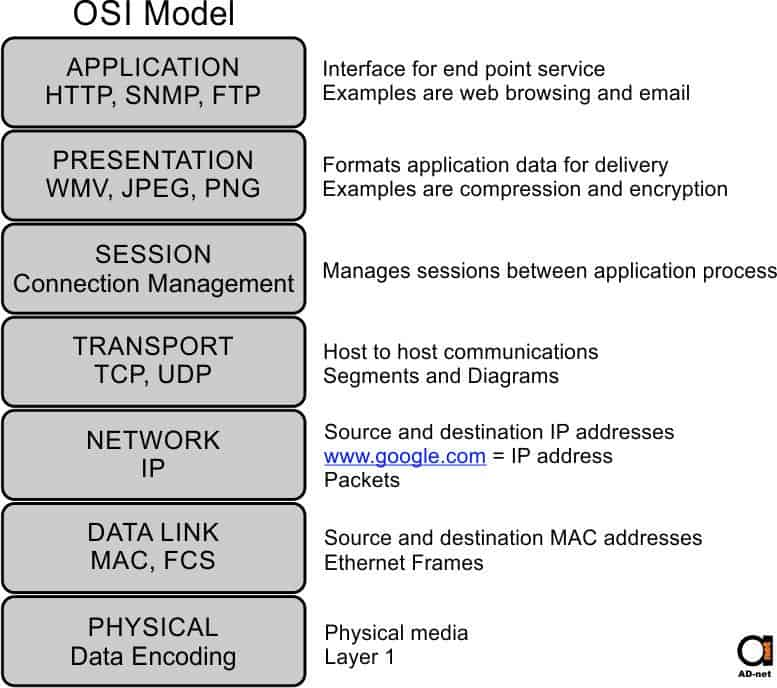
\includegraphics[width=\linewidth]{Images/osi.jpg}
                \tiny{https://www.ad-net.com.tw/osi-model-tcp-ip-network-models-must-concept-understand-move-deeper-networking-adventures/}
            \end{column}
            \begin{column}{.6\textwidth}
                \begin{itemize}
                    \item Hyper Text Transfer Protocol
                    \item OSI 7계층중 최상위 계층에 속하는 프로토콜
                    \item 주로 웹 브라우저와 웹 서버 사이에서의 통신에서 사용
                \end{itemize} 
            \end{column}
        \end{columns}
    \end{frame}

    \begin{frame}{HTTP와 OSI 7계층}
        \begin{center}
            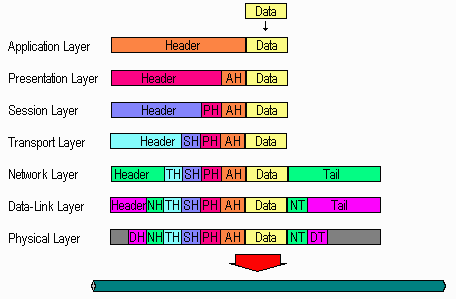
\includegraphics[width=\textheight]{Images/osidata_encap.png}
            \tiny{http://www.interfacebus.com/Design\_OSI\_Stack.html}
        \end{center}
    \end{frame}

    \begin{frame}{HTTP 패킷 구조}
        \begin{itemize}
            \item HTTP 패킷 = 헤더 + 데이터 (택배 상자)
            \item 헤더 = 보내고자 하는 데이터에 대한 설명 (택배 송장)
            \item 데이터 = 실제로 전송하고자 하는 데이터 (물건)
            \item 요청과 응답시 헤더가 조금씩 다름
        \end{itemize}
    \end{frame}

    \begin{frame}{HTTP 패킷 구조}
        \begin{columns}
            \begin{column}{.5\textwidth}
                \begin{center}
                    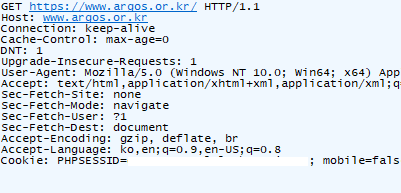
\includegraphics[width=\textwidth]{Images/request_http.png} 
                \end{center}
                
                \begin{itemize}
                    \item 요청 패킷 (GET)
                \end{itemize}                
            \end{column}
            \begin{column}{.5\textwidth}
                \begin{center}
                    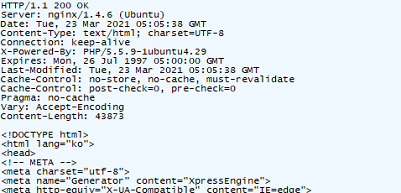
\includegraphics[width=\textwidth]{Images/response_http.png} 
                \end{center}
                \begin{itemize}
                    \item 응답 패킷
                \end{itemize}
            \end{column}
        \end{columns}
    \end{frame}

    \begin{frame}{클라이언트와 서버}
        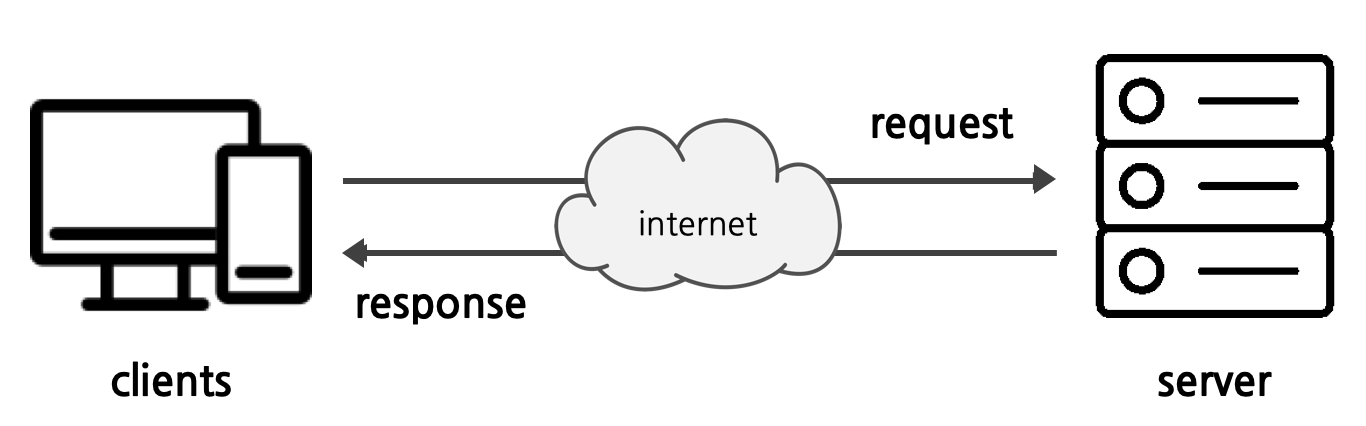
\includegraphics[width=\textwidth]{Images/server-client.jpg}
        \begin{itemize}
            \item 메일서버: 메일 (SMTP, IMAP 등) 관련 처리에 특화된 서버
            \item 게임서버: 게임 프로토콜 처리에 특화된 서버
            \item 웹서버: 웹 (특히 HTTP 요청) 관련 처리에 특화된 서버
        \end{itemize}
    \end{frame}

    \begin{frame}{HTTPS? TLS?}
        \begin{center}
            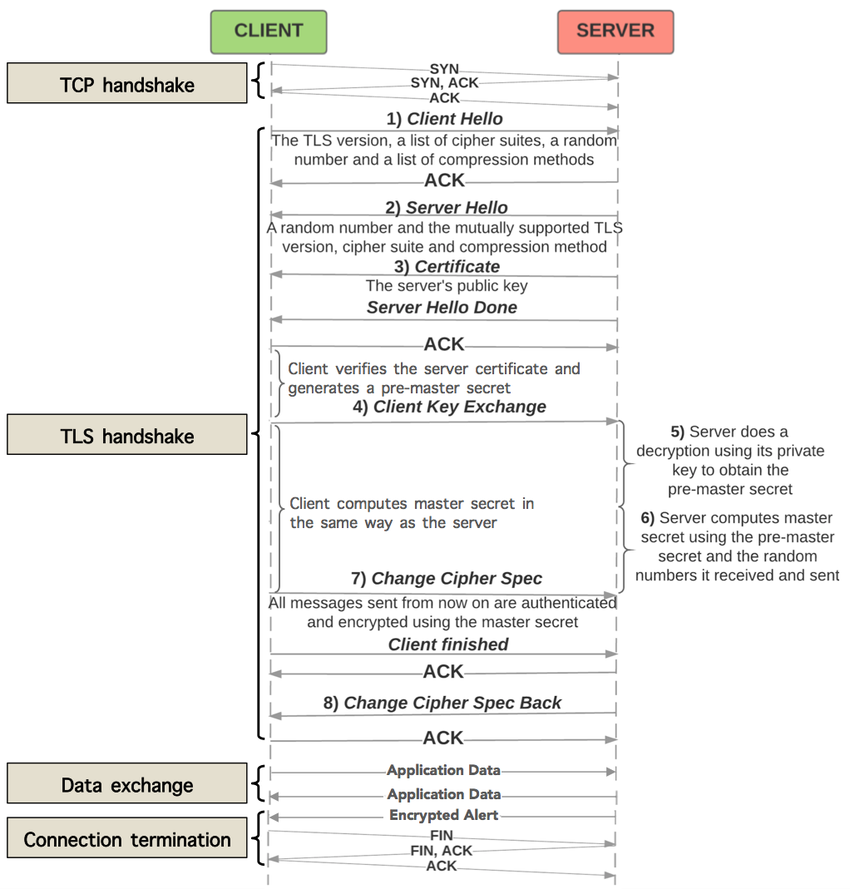
\includegraphics[height=0.7\textheight]{Images/https_seq.png}
            \tiny{\\https://www.researchgate.net/figure/HTTPS-message-sequence-diagram-with-detailed-TLS-handshaking-steps\_fig1\_306187575}
        \end{center}
    \end{frame}

\section{HTML과 PHP}
    \begin{frame}[fragile]
        \frametitle{HTML : 웹페이지의 구조를 설명하는 언어}
        \begin{itemize}
            \item Hyper Text Markup Language
            \item 프로그래밍 언어가 아님!
        \end{itemize}
    \end{frame}

    \begin{frame}[fragile]
        \frametitle{HTML 문서의 기본 구조}

        \begin{center}
            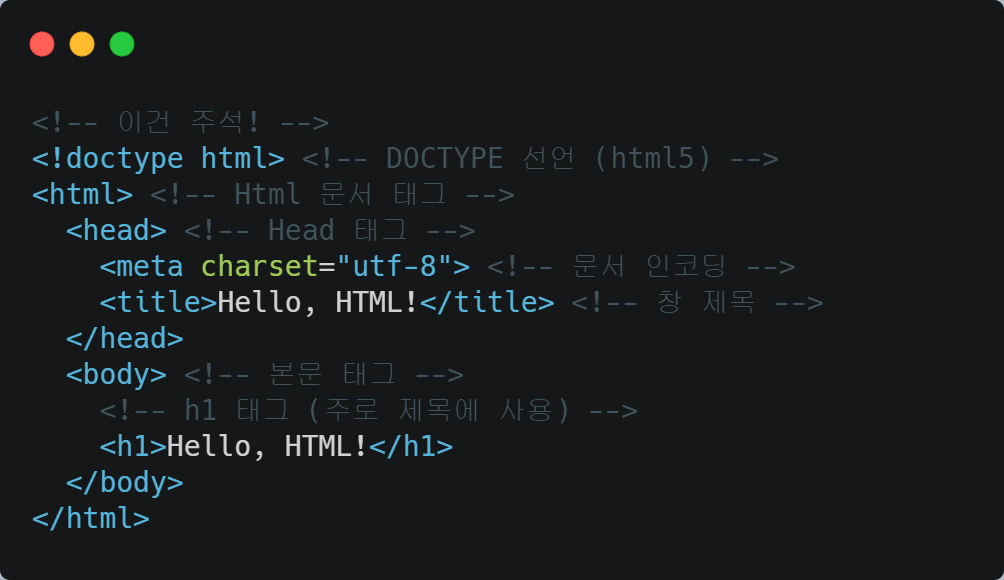
\includegraphics[height=0.7\textheight]{Images/structure-html.png}
        \end{center}
        
    \end{frame}

    \begin{frame}{주로 사용할 태그들}
        \begin{itemize}
            \item \texttt{html, head, body} : HTML 문서를 정의할때 필요
            \item \texttt{title} : 문서의 제목 설정
            \item \texttt{link} : 주로 CSS를 불러올 때 사용
            \item \texttt{script} : 자바스크립트를 불러오거나 작성할 때 사용
            \item \texttt{h1,h2, ..., h6} : 제목을 표현하는 태그
            \item \texttt{p} : 문단을 표현하는 태그
            \item \texttt{a} : 링크를 표현하는 태그
            \item \texttt{img} : 이미지를 불러올 때 사용
            \item \texttt{table, tr, td} : 표를 표현하는 태그
            \item \texttt{form, input} : 폼을 표현하는 태그 (제일 중요)
        \end{itemize}
    \end{frame}

    \begin{frame}{PHP}
        \begin{itemize}
            \item HTML은 기본적으로 정적(static)한 페이지를 작성
            \item 때로는 동적인 페이지가 필요 (e.g. 로그인 여부 확인, 게시글 표시 등...)
            \item 상황에 따라 페이지가 생성되어야 함!
        \end{itemize}
    \end{frame}

    \begin{frame}{PHP in HTML}
        \begin{itemize}
            \item \texttt{<?} 나 \texttt{<?php} 를 사용하여 코드 영역 시작
            \item 코드 영역을 끝낼때는 \texttt{?>}
            \item 파일 확장자는 \texttt{.php}
        \end{itemize}
        
        \begin{center}
            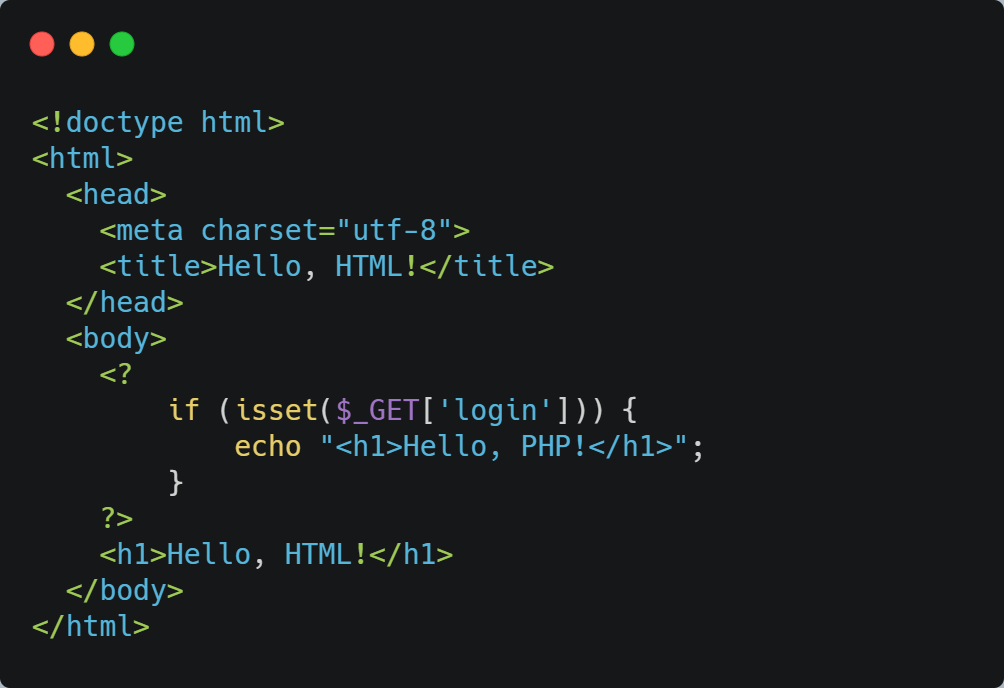
\includegraphics[height=0.5\textheight]{Images/html-php.png}
        \end{center}
    \end{frame}

    \begin{frame}{PHP의 동작 방식}
        \begin{center}
            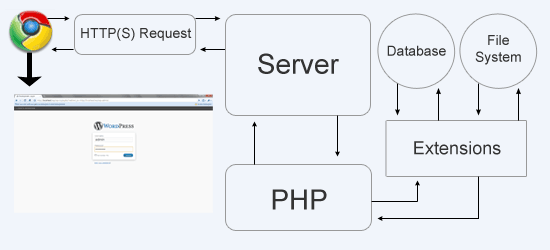
\includegraphics[width=\textwidth]{Images/how-php-works.png}
            \tiny{http://nepsdotin.github.io/php-tutorial/site/unit-3/how-php-works/}
        \end{center}
        
    \end{frame}

    \begin{frame}{여태까지 내용 정리하기}
        \begin{itemize}
            \item HTTP를 처리하는 서버는 웹 서버
            \item 웹 문서를 작성하는 언어 HTML
            \item 동적 페이지를 작성하는 언어 PHP
            \item 웹서버가 PHP 요청을 받으면 PHP 인터프리터로
            \item PHP 인터프리터의 실행 결과는 웹서버를 거쳐 사용자로
        \end{itemize}
    \end{frame}

\section{개발환경 구축하기}
    \begin{frame}{JetBrains PHPStorm}
        \begin{columns}
            \begin{column}{0.4\textwidth}
                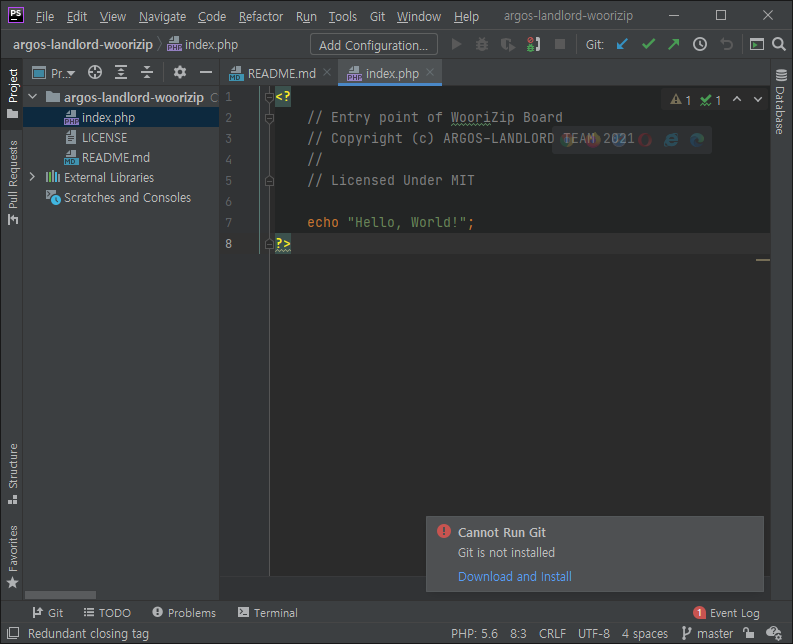
\includegraphics[width=\textwidth]{Images/jetbrains-0.png}
            \end{column}
            \begin{column}{0.6\textwidth}
                \begin{itemize}
                    \item PHP 개발에 필요한 편의기능 제공
                    \item 라이브 서버, 인텔리센스, 패키지관리 등...
                    \item 학교 이메일로 무료 사용가능
                \end{itemize}
            \end{column}
        \end{columns}
    \end{frame}

    \begin{frame}{PHP 디버그 환경 설정}
        \begin{itemize}
            \item Windows: windows.php.net
            \item Linux: 각 패키지 매니저별 설치방법 참조
            \item OSX: ???
        \end{itemize}
    \end{frame}

    \begin{frame}{인텔리센스나 이런저런 도움이 필요 없다면...}
        \begin{itemize}
            \item Visual Studio Code를 써도 됩니다!
            \item PHP Server 확장기능: 라이브 서버가 필요할 경우
            \item 단 직접 경로 잡고 세팅해야함!
            \item 제대로 세팅하지 않으면 인텔리센스가 많이 불편
        \end{itemize}
    \end{frame}

\section{PHP 기초}
    \begin{frame}{\texttt{echo "Hello, World!"}}
        \begin{itemize}
            \item 문자열 출력은 \texttt{echo}를 사용
        \end{itemize}
        \begin{center}
            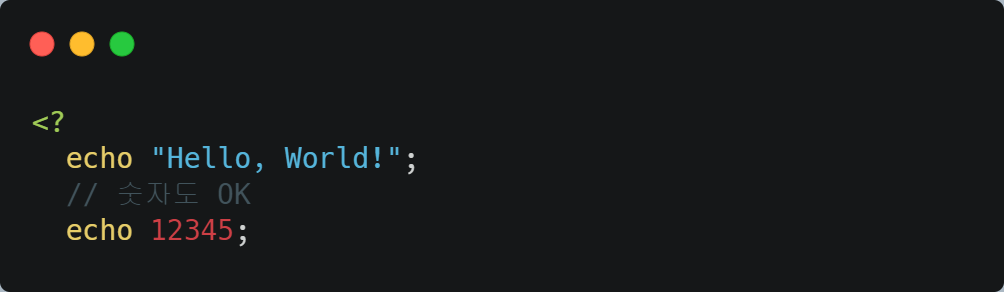
\includegraphics[width=\textwidth]{Images/php1.png}
        \end{center}
    \end{frame}

    \begin{frame}{변수 선언}
        \begin{itemize}
            \item PHP에서 모든 변수는 \texttt{\$} 로 시작한다
        \end{itemize}
        \begin{center}
            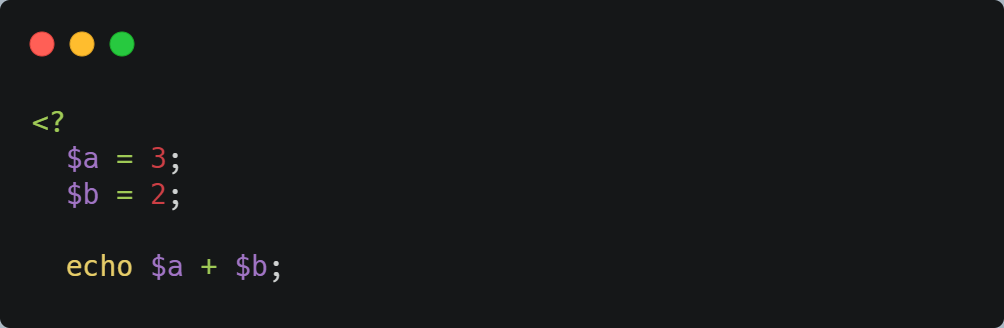
\includegraphics[width=\textwidth]{Images/php2.png}
        \end{center}
    \end{frame}

    \begin{frame}{이런저런 문자열 다루기}
        \begin{itemize}
            \item 큰 따옴표, 작은 따옴표 모두 문자열
                  
            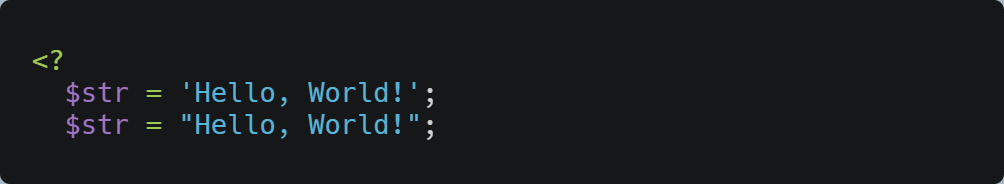
\includegraphics[height=0.1\textwidth]{Images/php3.png}
            \item 문자열을 int로
                  
            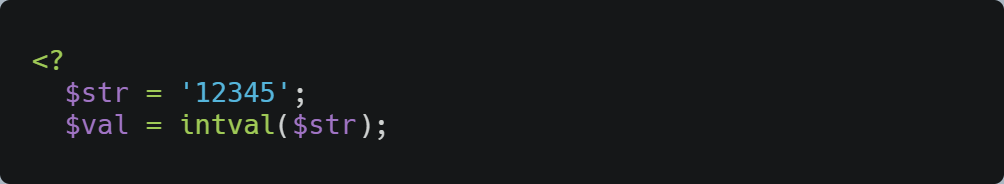
\includegraphics[height=0.1\textwidth]{Images/php4.png}
            \item 두 스트링끼리 붙일 땐 \texttt{.}
                  
            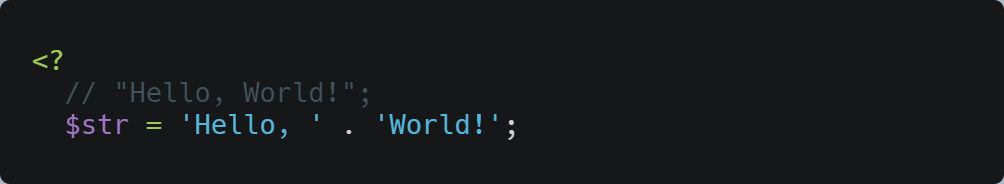
\includegraphics[height=0.1\textwidth]{Images/php5.png}
            \item 큰 따옴표에서는 문자열에 변수 삽입(interpolation) 가능
                  
            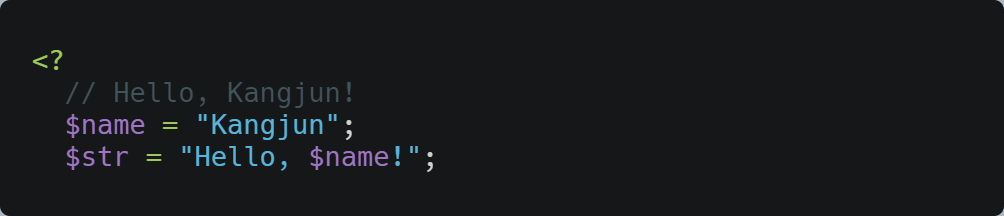
\includegraphics[height=0.1\textwidth]{Images/php6.png}
        \end{itemize}
    \end{frame}

    \begin{frame}{특별한 변수들: Superglobals}
        \begin{itemize}
            \item \texttt{\$\_GET} : GET 파라메터를 담는 전역변수
            \item \texttt{\$\_POST} : POST 파라메터를 담는 전역변수
            \item \texttt{\$\_FILES} : POST로 날아온 파일 정보를 담는 전역변수
            \item \texttt{\$\_SERVER} : 서버 환경설정, 클라이언트 연결 정보를 담는 전역변수
        \end{itemize}
    \end{frame}

    \begin{frame}{GET? POST?}
        \begin{itemize}
            \item HTTP 메서드의 일종
            \item 메서드에 따라 백엔드로 데이터를 전달하는 방법이 다름
            \item 데이터가 주소에 실려있다? \texttt{\$\_GET} 에 할당
            
            e.g.) \texttt{http://example.com/index.php?page=100}
            \item 데이터가 패킷에 실려있다? \texttt{\$\_POST} 에 할당
            \item 자세한 내용은 2주차에!
        \end{itemize}
    \end{frame}

    \begin{frame}{연산자들}
        \begin{itemize}
            \item C나 자바에서 사용하는것과 거의 동일!
            
            \item 대입: \texttt{=}
            \item 산술연산자: \texttt{+, -, \*, /, <<, >>, \&, |}
            \item 논리연산자: \texttt{==, ===, !=, !==, <, > \&\&, ||}
            \item 증감연산자: \texttt{++, --}
            \item 문자열연결: \texttt{.}
        \end{itemize}
    \end{frame}

    \begin{frame}{제어문, 반복문}
        \begin{itemize}
            \item \texttt{if, switch, while, for, foreach}\dots
            \item C나 자바와 마찬가지로 사용
        \end{itemize}
        \begin{center}
            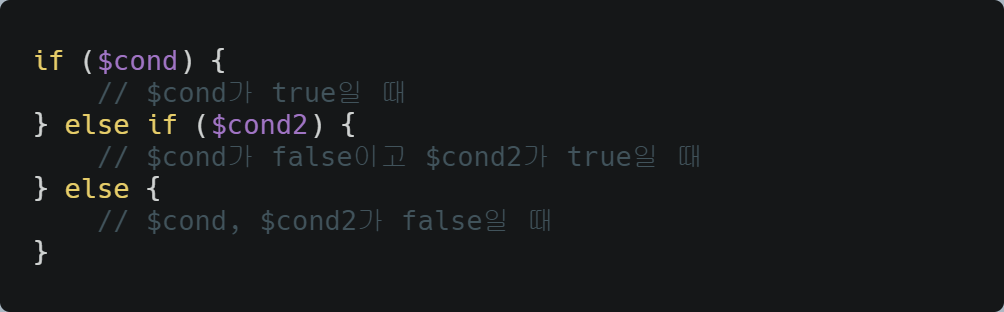
\includegraphics[height=0.45\textheight]{Images/php11.png}
        \end{center}
    \end{frame}

    \begin{frame}{제어문, 반복문}
        \begin{center}
            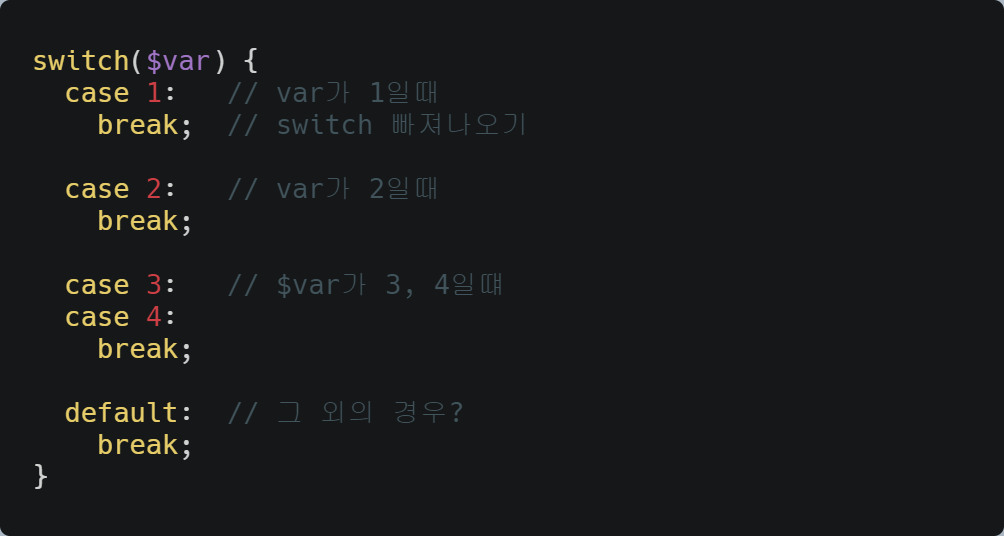
\includegraphics[width=\textwidth]{Images/php12.png}
        \end{center}
    \end{frame}

    \begin{frame}{제어문, 반복문}
        \begin{center}
            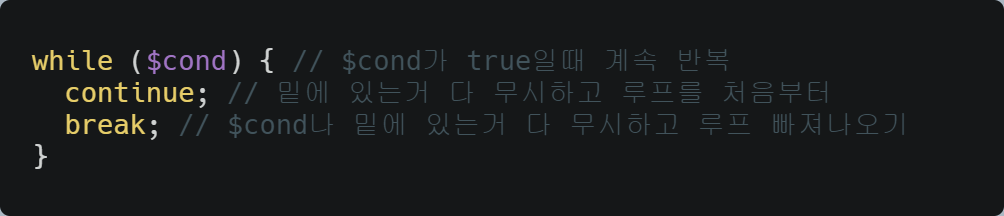
\includegraphics[width=\textwidth]{Images/php13.png}
        \end{center}
    \end{frame}

    \begin{frame}{제어문, 반복문}
        \begin{center}
            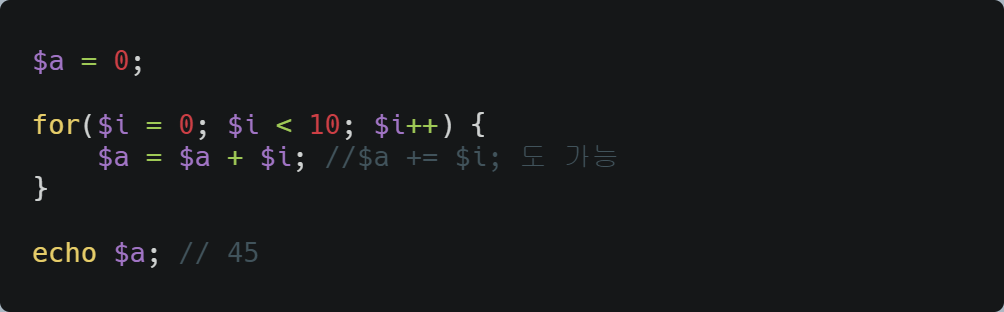
\includegraphics[width=\textwidth]{Images/php14.png}
        \end{center}
    \end{frame}

    \begin{frame}{제어문, 반복문}
        \begin{center}
            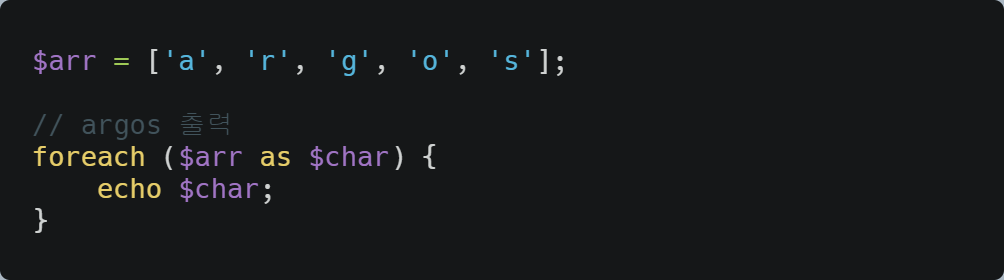
\includegraphics[width=\textwidth]{Images/php15.png}
        \end{center}
    \end{frame}

    \begin{frame}{변수나 요소가 있는지 검사하기}
        \begin{itemize}
            \item \texttt{isset} 함수: 특정 변수가 선언되었는지 검사하기
        \end{itemize}
        \begin{center}
            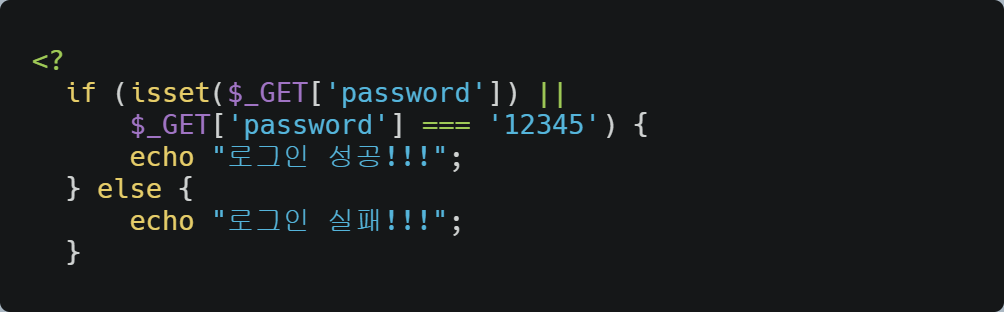
\includegraphics[width=\textwidth]{Images/php9.png}
        \end{center}
    \end{frame}

    \begin{frame}{함수 정의 및 호출}
        \begin{itemize}
            \item \texttt{function} 키워드를 이용해 정의
            \item \texttt{()}연산자를 이용해 호출
        \end{itemize}
        \begin{center}
            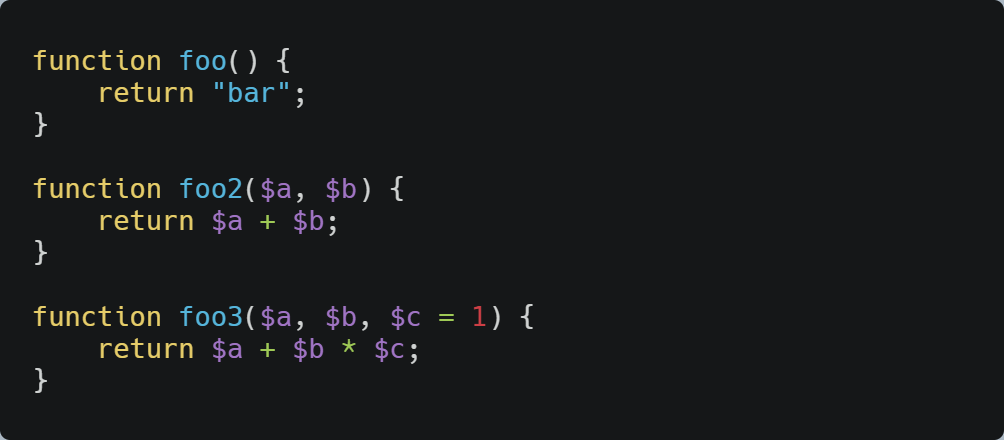
\includegraphics[height=0.4\textheight]{Images/php10.png}
        \end{center}
    \end{frame}

\section{마무리}
    \begin{frame}{실습: Hello, landlord!}
        \begin{itemize}
            \item echo 문을 이용해서 Hello, (이름) 을 출력해보세요.
            \item \underline{변수를 이용}해볼 것!
            \item \underline{String Interpolation}을 이용할 것!
            \item 파일명은 \texttt{hello.php} 로 (브라우저로 접속 가능해야함)
            \item 기한: 다음주 활동시간까지
        \end{itemize}
    \end{frame}

    \begin{frame}{Project: WooriZip Board : 게시판 만들기}
        \begin{itemize}
            \item 웹 서비스에서 가장 많이 사용되는 유형의 프로그램
            \item CRUD (Create, Read, Update, Delete)를 학습하기 좋음
            \item 프로그램 크기도 적당히 크기 때문
            \item 진도 나가면서 매주 기능 하나하나 구현해보기!
        \end{itemize}
    \end{frame}

    \begin{frame}{질문?}

    \end{frame}

\end{document}